\documentclass{article}

% if you need to pass options to natbib, use, e.g.:
%     \PassOptionsToPackage{numbers, compress}{natbib}
% before loading neurips_2024


% ready for submission
\usepackage{neurips_2024}
\usepackage{algorithm,algpseudocode}
\usepackage{amsmath}
\usepackage{graphicx}
\usepackage{caption}
\usepackage{subcaption}

\graphicspath{ {./images/} }


% to compile a preprint version, e.g., for submission to arXiv, add add the
% [preprint] option:
%     \usepackage[preprint]{neurips_2024}


% to compile a camera-ready version, add the [final] option, e.g.:
%     \usepackage[final]{neurips_2024}


% to avoid loading the natbib package, add option nonatbib:
%    \usepackage[nonatbib]{neurips_2024}


\usepackage[utf8]{inputenc} % allow utf-8 input
\usepackage[T1]{fontenc}    % use 8-bit T1 fonts
\usepackage{hyperref}       % hyperlinks
\usepackage{url}            % simple URL typesetting
\usepackage{booktabs}       % professional-quality tables
\usepackage{amsfonts}       % blackboard math symbols
\usepackage{nicefrac}       % compact symbols for 1/2, etc.
\usepackage{microtype}      % microtypography
\usepackage{xcolor}         % colors


\title{Final Report for CSE561 Fall 2024}


% The \author macro works with any number of authors. There are two commands
% used to separate the names and addresses of multiple authors: \And and \AND.
%
% Using \And between authors leaves it to LaTeX to determine where to break the
% lines. Using \AND forces a line break at that point. So, if LaTeX puts 3 of 4
% authors names on the first line, and the last on the second line, try using
% \AND instead of \And before the third author name.


\author{%
  David S. Hippocampus\thanks{Use footnote for providing further information
    about author (webpage, alternative address)---\emph{not} for acknowledging
    funding agencies.} \\
  Department of Computer Science\\
  Cranberry-Lemon University\\
  Pittsburgh, PA 15213 \\
  \texttt{hippo@cs.cranberry-lemon.edu} \\
  % examples of more authors
  % \And
  % Coauthor \\
  % Affiliation \\
  % Address \\
  % \texttt{email} \\
  % \AND
  % Coauthor \\
  % Affiliation \\
  % Address \\
  % \texttt{email} \\
  % \And
  % Coauthor \\
  % Affiliation \\
  % Address \\
  % \texttt{email} \\
  % \And
  % Coauthor \\
  % Affiliation \\
  % Address \\
  % \texttt{email} \\
}


\begin{document}


\maketitle


\begin{abstract}

    We introduce Flow of Thoughts, a novel framework that enables large language models (LLMs) to effectively process and reason about long passages by combining self-RAG based generation with knowledge graph construction. The framework dynamically builds and traverses a knowledge graph while solving problems, allowing flexible information retrieval and aggregation. Through independent solution paths with built-in self-verification, Flow of Thoughts achieves competitive performance compared to existing approaches like Graph of Thoughts, particularly excelling at tasks requiring synthesis of information from large texts. Our experiments on sorting, set intersection, and reading comprehension demonstrate the framework's effectiveness across different problem domains. Website and code are available at \url{https://github.com/Trance-0/Flow-of-Thoughts}.

\end{abstract}


\section{Introduction}

This final project investigates novel approaches to enhance how Large Language Models (LLMs) store, manage, and retrieve knowledge and references. Recent research has shown that LLMs inherently act as natural compressors of information \cite{delétang2024languagemodelingcompression}. Building on this insight, we propose efficiently representing knowledge as graph nodes annotated with semantic tag tuples, enabling flexible and contextual retrieval. This graph-based approach allows us to scale to large amounts of data while maintaining the ability to surface relevant information during inference.

A fundamental challenge with LLMs is their limited ability to effectively utilize long-range context. Studies have revealed that LLMs exhibit a distinctive U-shaped performance pattern based on information positioning - they perform optimally when critical information appears either at the beginning (primacy effect) or end (recency effect) of the input context, but struggle significantly when important details are embedded in the middle \cite{liu2023lostmiddlelanguagemodels}. This "lost in the middle" phenomenon poses a significant barrier to processing longer documents.

Also, LLMs are prone to generating hallucinations when solving problems. They may generate incorrect or fabricated statements that snowball into more errors \cite{zhang2023languagemodelhallucinationssnowball}, making the model overconfident in its own answers, especially when the input is long. The credibility of the model's responses will be lost along long induction chains and retrieval processes.

This limitation becomes particularly problematic when considering real-world applications, where problem-solving often requires synthesizing information from multiple sources and considering various aspects simultaneously. Just as human experts draw upon extensive knowledge bases to make informed decisions, LLMs need mechanisms to efficiently access and reason over large bodies of information. While simply increasing context window sizes offers one potential solution, we argue that more sophisticated approaches to knowledge management and retrieval are essential for enabling LLMs to achieve human-like reasoning capabilities across complex, information-rich domains.

\section{Related work}
% Related work (an extended one if the related work in your proposal does not discuss specific approaches directly related to your problem setting)

\subsection{Chain-of-thoughts}

Chain-of-thoughts \cite{Wei2022ChainOT} is an effective prompting method discovered in 2023 by Jason Wei et al. It provides an example of a logic chain to solve a problem similar to the target question, allowing the LLMs to think step by step. This prompt can be used in the Training and Prompting stage of the LLM and generally provides better results when dealing with problems in Mathematics and Engineering.

One significant constraint faced by LLMs based on CoT is the context window size. This can lead to situations where the model forgets previous steps when working through complex problems, particularly in scenarios that require Chain-of-Thought (CoT) reasoning.

\subsection{Graph-of-thoughts}

Graph of thoughts \cite{Besta_2024} is a framework used to prompt LLMs by collecting the thinking process and branching different ideas generated by LLMs. Using generation and aggregation, the model selects the best result in the thinking process and develops from that.  

Integrating concepts such as the Graph of Thoughts and other search methods might provide valuable support for solving problems with a limited context window. By employing these techniques, we can enhance the model's ability to organize and retrieve relevant data, facilitating better problem-solving even with constrained memory resources.

However, during the aggregation process, the LLM cannot freely choose the information they need to solve the problem but must propagate from previous thoughts. In this research, our framework will try to give the LLM the ability to choose the material that they find helpful.

\subsection{Express uncertainty}

Another relevant approach is detailed in a paper discussing the certainty of LLMs in problem-solving \cite{lin2022teachingmodelsexpressuncertainty}. This research focuses on how models express and handle uncertainty, which can be instrumental in determining when to terminate the search or prompting process. Specifically, the authors explore techniques such as uncertainty sampling and confidence thresholds, which allow models to quantify their level of certainty about generated outputs. Understanding and incorporating measures of certainty can help optimize when and how the model utilizes its context, thereby allowing it to defer to more reliable responses or request additional information when faced with ambiguous queries. Understanding and incorporating measures of certainty can help optimize when and how the model utilizes its context, potentially leading to more accurate and efficient problem-solving.

\subsection{Self-verification}

Self-verification \cite{weng2023largelanguagemodelsbetter} is an important technique in improving the reliability of responses generated by large language models (LLMs). When an LLM initially produces an answer, there may be some inaccuracies due to the model's limitations in understanding the full context or providing detailed reasoning. However, the model has the ability to correct or refine its output by "thinking twice." One way this can be achieved is by prompting the model to reverse the roles of questions and answers. By taking the original answer and transforming it back into a question, followed by asking the LLM to generate an updated or revised answer, researchers can often obtain a more accurate and thoughtful response.

This process encourages the model to evaluate its earlier reasoning and detect inconsistencies or gaps in logic that may have been overlooked initially. The technique leverages the model's own knowledge to reassess and validate its responses, thereby functioning as a form of internal feedback. Additionally, this self-verification approach may prompt the model to consider alternative interpretations of the question, helping to mitigate issues like oversimplification or misunderstanding of complex queries. By iterating in this manner, the quality of the response can be significantly enhanced, offering a more reliable and nuanced answer for the user.

\subsection{Memorizing Transformers and Self-Reflective Retrieval-Augmented Generation (SELF-RAG)}

Furthermore, exploring memorizing transformers and their approaches could provide additional strategies for extending Transformer architectures using kNN \cite{wu2022memorizingtransformers}. These methods focus on enhancing the model's ability to retain and recall information across longer contexts, potentially offering practical solutions for memory limitations.

Other frameworks like Self-RAG \cite{asai2023selfraglearningretrievegenerate} are also helpful for LLMs to retrieve essential information when solving problems in long paragraphs. The model incorporates a feedback loop where it reflects on its own generated responses to improve their quality before delivering them. This reflection can involve: checking for consistency with the retrieved documents, verifying the factual accuracy, and identifying potential hallucinations (when the model generates incorrect or fabricated information).

\section{Framework design}
% (highlight the contribution of your method: novelty/effectiveness/efficiency/simplicity)

We propose a novel Flow of Thoughts framework that can dynamically process and reason about long passages using self-RAG based generation combined with knowledge graph construction. This framework enables large language models to effectively manage and utilize information from extensive texts while maintaining coherent logic chains. The framework consists of four main components:

\subsection{Preprocessing}

First, the LLM constructs a knowledge graph by splitting input long passages into syntactically and semantically independent units that fit within the model's context window.

For academic papers, this involves breaking down the text into logical sections such as abstract, introduction, related work, methodology, and results. Each section is further subdivided if needed to ensure it fits within context limits while preserving meaningful relationships. For reading comprehension tasks, the framework segments passages into coherent paragraphs that maintain narrative flow and topical consistency while staying within context window constraints.

The model can also use predefined knowledge graphs as well.

\subsection{Generating methods}

The framework then employs a multi-strategy approach by having the LLM generate diverse solution methods tailored to the specific problem type. For example, when tackling sorting problems, the LLM generates multiple sorting algorithms like bubble sort, quick sort, and merge sort. 

For each method, the LLM also performs an error analysis by identifying potential pitfalls and edge cases that could arise during execution for future refinement.

\subsection{Self-verification and refining}

On each branch of the solution, the framework feeds the problem statement, generated methods, and data corpus to the LLM. The model evaluates passage relevance and uses the generated methods to solve the problem. The LLM will also check if the generated thought follows the generated methods and the problem statement using self-verification \cite{weng2023largelanguagemodelsbetter}. To achieve this, we provide the LLM with the method description and generated output, we ask the LLM to self-verify the output and the method and capture the mistakes as we go.

Then, we ask the LLM to iteratively check the list of potential mistakes that was generated in the previous steps.

If new errors are found, we may also add the new errors to the checking process.

For instance, when answering questions about technical approaches used in a project, the LLM selectively focuses on relevant sections like "Related Work" while appropriately discounting less relevant sections like conclusions or experimental results. This targeted attention mechanism helps maintain solution quality while managing computational resources effectively.

Ideally, in this step, the LLM should take control of the thought generation and refinement process and should be able to determine the steps required to solve the problem. However, in this research, we don't have sufficient time to implement such a protocol, which can be done in the future. \ref{sec:future_work_self_generation}

\subsection{Aggregation}

The final phase aggregates the final thoughts from each independent branch to reach the final answer. Unlike Graph of Thoughts approaches that merge partial solutions, our framework uses a majority voting system to determine the final answer.

\begin{algorithm}
    \caption{Flow of thoughts($P,Q$)}\label{alg:cap}
    \begin{algorithmic}
        \Require Generator LM $\mathcal{M}$
        \Require Large-scale passage collections $P=\{d_1, . . . , d_N \}$
        \Require Final question $Q$.
        \Require Predefined root thought node that contains the problem statement $problem\_root$
        \State $methods\gets LM(\text{How to solve the problem } Q, \text{number of methods})$
        \Comment{Generate methods to solve the problem}
        \State $solutions\gets []$
        \For{each $method \in methods$}
            \State $segments \gets []$
            \State $mistakes\gets LM(\text{common mistakes in } method)$
            \Comment{Extract segments from the knowledge graph to obtain relevant information}
            \While {$P$ is not empty}
                    \State $current\_passage\gets P.pop()$
                    \State $current\_segment\gets \mathcal{M}($ relevant info in $current\_passage$ to solve problem $Q))$
                \If{current\_segment is not empty}
                    \State $segments.\text{add}(current\_segment)$
                \EndIf
            \EndWhile
            \State $thoughts\gets[problem\_root]$
            \Comment{Aggregate the segments to form a rudimental solution}
            \For{ each $current\_segment\in segments$}
                \State $thoughts.\text{add}(current\_segment)$
            \EndFor
            \While {$thoughts.size()>1$}
                \State $thought\gets thoughts.pop()$
                \For{each $operation \in thought.child\_operations$}
                    \State $operation.execute()$
                    \Comment{Execute the operation with various types, such as retrieval, generation, etc. We can capture the mistakes and refine the solution on execution steps.}
                    \For{each $child\_thoughts \in operation.child\_thoughts$}
                        \If{$child\_thoughts.is\_executable()$}
                            \State $thoughts.\text{add}(child\_thoughts)$
                        \EndIf
                    \EndFor
                \EndFor
            \EndWhile
            \State $solutions.\text{add}(thoughts)$
        \EndFor
        \State \Return $majority(solutions)$

        
    %%%%%%%%%%%%%%%%%%%%%%%%%%%%%%%%%%%%%%%%%%%%%%%%%
    % page breaking algorithm block
    % \algstore{myalg}
    % \end{algorithmic}
    % \end{algorithm}
    % \clearpage
    % \begin{algorithm}
    % % don't forget to add your name of algorithm here
    % \caption{Have safe range ($P$) (continued)}
    % \begin{algorithmic}
    % \algrestore{myalg}
    % page breaking algorithm block
    %%%%%%%%%%%%%%%%%%%%%%%%%%%%%%%%%%%%%%%%%%%%%%%%
    \end{algorithmic}
    \end{algorithm}
    \begin{figure}[h]
        \centering
        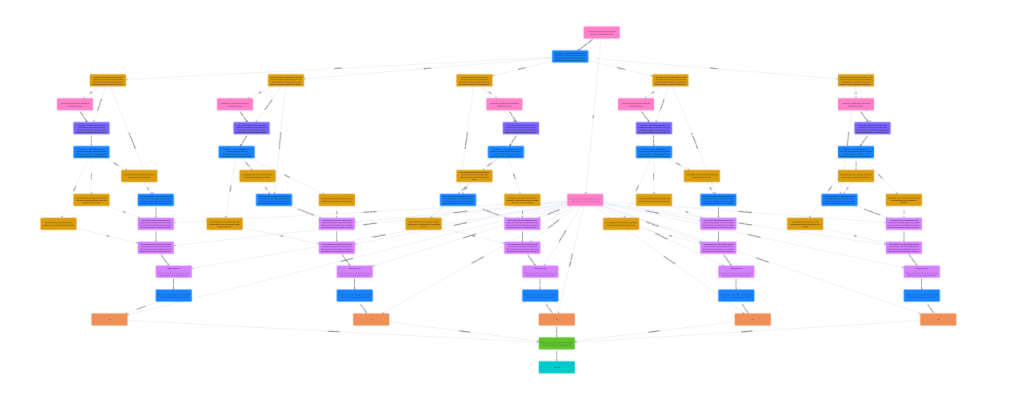
\includegraphics[width=1.0\textwidth]{images/flow_of_thoughts.png}
        \caption{Flow of Thoughts framework using graph visualization, the pink nodes are the nodes from the knowledge graph or definition of the problem, the yellow nodes are generated by the LLM, the purple nodes are refinement of the solution generated by the LLM. In the final layer, the LLM will aggregate the solution and generate the final answer (the cyan node)}
        \label{fig:flow_of_thoughts}
    \end{figure}

    The framework is designed to be a general framework that can be applied to any problem that can be solved by LLMs.

\subsection{Novelty of the solution}

The Flow of Thoughts framework introduces a new approach to processing and extracting relevant information from a large data corpus that might contain the necessary information to solve the target problem using Self-RAG and a Graph of Thoughts structure, significantly enhancing the efficiency, relevance, and quality of interactions with long-form content. 

This model provides more explainability by recording how LLMs get the final solution from aggregating the partial information gained from Self-RAG. Through the segmentation, contextual relevance filtering, and ability to compose well-supported answers, this framework can potentially stand out in the landscape of text processing and information retrieval technologies.

\subsection{Efficiency}

Compared with a normal Graph of Thoughts, the framework proposes independent approaches to solve the problem and solves it automatically with self-checking for common mistakes and refines the solution along each step. This uses generation of LLM more effectively since each path is independent and the LLM can generate more diverse solutions compared to the normal Graph of Thoughts or Tree of Thoughts.

Moreover, the framework intelligently filters irrelevant sections based on the posed question and methods, enabling the model to focus solely on pertinent information. This specificity enhances the accuracy of the responses generated by the LLM and saves costs when dealing with large data corpus.

Compared with a normal Self-RAG Inference, the framework provides more flexibility for the convergence of information for black-boxed models like ChatGPT and Claude. It's easier to migrate to a new model without training the retriever and fine-tuning costs.

\subsection{Effectiveness}

The framework is designed to be a general framework that can be applied to most of the problems that can be solved by LLMs. All the prompts and methods are generated by the LLM itself; we only need to provide few-shot examples to guide the LLM to generate the prompts and methods in our setting. In later experiments, we observed that our scheme is competitive with Graph of Thoughts and even outperforms it in some cases.

\section{Experiment results}

To test the performance of the Flow of Thoughts framework, we have implemented basic functions for the Flow of Thoughts in revised Graph of Thoughts framework with implementation of basic input and output (IO), Chain-of-Thought (CoT), Tree-of-Thought (ToT), Graph-of-Thought (GoT), and Flow-of-Thought (FoT). All the prompts are given with 3-shot examples. For the flow of thoughts framework, the shots are given three simple tasks with potential approaches.

We use black-box models GPT-4o-mini and Claude-3.5-Sonet with API calls for the experiment. For both models, we set temperature to 0.7 with all other parameters to default.

\begin{figure}[h]
    \centering
    \begin{subfigure}{0.15\textwidth}
        \centering
        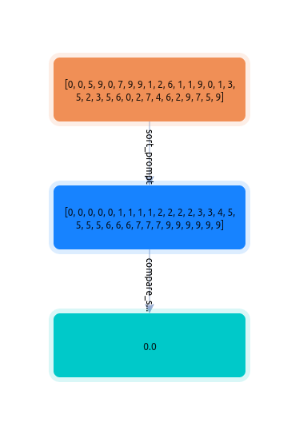
\includegraphics[width=0.5\textwidth]{images/io.png}
        \subcaption{IO}
    \end{subfigure}%
    \begin{subfigure}{0.15\textwidth}
        \centering
        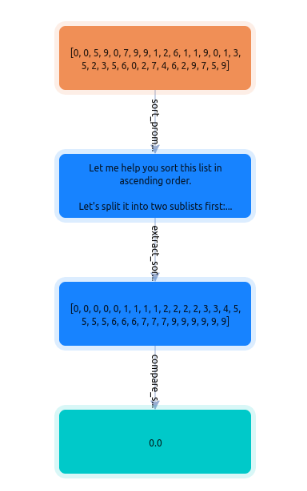
\includegraphics[width=0.5\textwidth]{images/chain_of_thoughts.png}
        \subcaption{CoT}
    \end{subfigure}%
    \begin{subfigure}{0.7\textwidth}
        \centering
        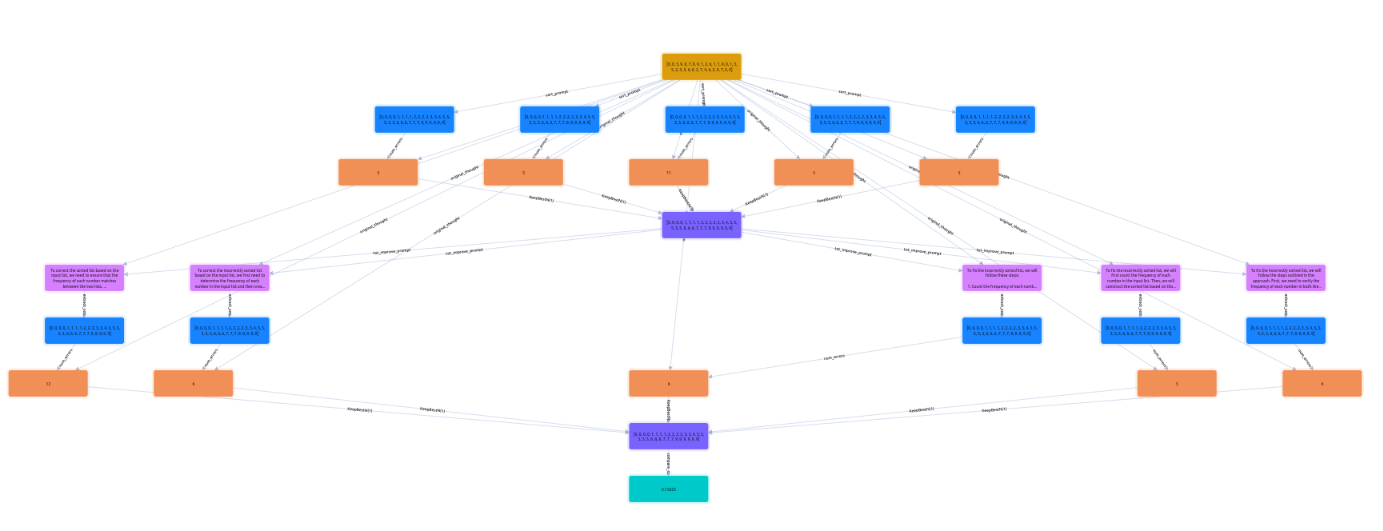
\includegraphics[width=1.0\textwidth]{images/tree_of_thoughts.png}
        \subcaption{Tree-of-Thought scheme}
    \end{subfigure}
    \begin{subfigure}{1.0\textwidth}
        \centering
        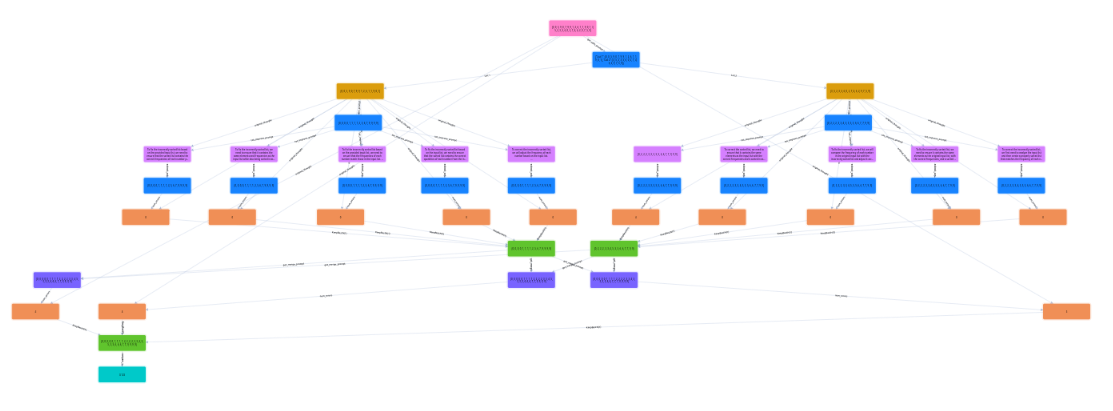
\includegraphics[width=1.0\textwidth]{images/graph_of_thoughts.png}
        \subcaption{Graph-of-Thought scheme}
    \end{subfigure}
    \caption{Other framework structures defined in the experiment, only used for reference, detailed structure can be found in each run of the experiment}
    \label{fig:sorting_results}
\end{figure}

\subsection{Sorting}

The sorting task is a basic task that can be solved by Graph of Thoughts. We give the LLM a list of 32 random numbers and let each scheme sort the numbers. The number of trials is 100. The number of errors is calculated by the number of trials in which the LLM cannot sort the numbers correctly. Dataset can be found in appendix \ref{sec:appendix_sorting}.

All the prompts are given with 3-shot examples. For the flow of thoughts framework, the shots are given three simple tasks with potential approaches.

\begin{table}[h]
    \centering
    \begin{tabular}{|c|c|c|}
        \hline
        \textbf{Model} & \textbf{GPT-4o-mini} & \textbf{Claude-3.5-Sonet} \\
        \hline \hline
        \textbf{IO}    & 2.14                 & 2.03                     \\
        \textbf{CoT}   & 1.88                 & 1.86                     \\
        \textbf{ToT}   & 1.20                 & 1.32                     \\
        \textbf{GoT}   & 1.10                 & 1.32                     \\
        \textbf{FoT}   & 1.13                 & \textbf{1.09}                     \\
        \hline
    \end{tabular}
    \vspace{1em}
    \caption{Average number of incorrect responses in sorting 32 integers}
    \label{tab:sorting_results}
\end{table}

\subsection{Set Intersection}

The set intersection task is a basic task that also can be solved by Graph of Thoughts. The task is defined as follows: Given two sets of 32 numbers, find the intersection of the two sets.

We use the same dataset as the Graph of Thoughts and compare the performance with Graph of Thoughts. Dataset can be found in appendix \ref{sec:appendix_set_intersection}.

The experiment is conducted with 100 trials. The number of errors is calculated by the number of misclassified elements in the intersection.

\begin{table}[h]
    \centering
    \begin{tabular}{|c|c|c|}
        \hline
        \textbf{Model} & \textbf{GPT-4o-mini} & \textbf{Claude-3.5-Sonet} \\
        \hline \hline
        \textbf{IO}    & 3.02                 & 2.88                     \\
        \textbf{CoT}   & 2.46                 & 1.89                     \\
        \textbf{ToT}   & 1.93                 & 1.97                     \\
        \textbf{GoT}   & 1.24                 & 1.56                     \\
        \textbf{FoT}   & \textbf{1.13}                 & 1.20                     \\
        \hline
    \end{tabular}
    \vspace{1em}
    \caption{Average number of incorrect responses in set intersection}
    \label{tab:set_intersection_results}
\end{table}

\subsection{Reading Comprehension}

For the reading comprehension task, we use the RACE dataset \cite{lai2017large} to test the performance of the Flow of Thoughts framework. The dataset contains 28,000+ passages and 100,000+ questions, which is a large dataset for reading comprehension tasks. We use the subset of the top 100 longest passages to test the performance of the Flow of Thoughts framework. (min passage length 3850 words, details of the passages can be found in the appendix)

The experiment is conducted with 100 passages. Each passage weights 1 point and we calculate the total score of the model by summing up the scores of each passage. The best score obtained is 85.5, whereas the SOTA score is 91.4 by ALBERT (Ensemble)\cite{jiang2020improvingmachinereadingcomprehension}.

\begin{table}[h]
    \centering
    \begin{tabular}{|c|c|c|}
        \hline
        \textbf{Model} & \textbf{GPT-4o-mini} & \textbf{Claude-3.5-Sonet} \\
        \hline \hline
        \textbf{IO}    & 68.5                 & 65.25                    \\
        \textbf{CoT}   & 72.33                & 69.5                     \\
        \textbf{ToT}   & 76.25                & 75.33                    \\
        \textbf{GoT}   & 78.5                 & 83.25                    \\
        \textbf{FoT}   & 84.33                & \textbf{85.5}                     \\
        \hline
    \end{tabular}
    \vspace{1em}
    \caption{Score of the reading comprehension task on RACE-min dataset}
    \label{tab:reading_comprehension_results}
\end{table}

\section{Analysis}

\subsection{Method generation}

By default, we let the LLM generate 3 methods for each task all by themselves. However, the model may not be able to generate 3 practical methods that LLM can execute. 

For sorting task, in some rare cases, the LLM will generate methods using python code. However, in our setting, the LLM does not have the capability to execute python code and the methods will be processed as a normal tree of thoughts branch and don't contribute to the diversity of the solutions. This case is also observed in the set intersection task, where the LLM will also use \texttt{set.intersection()} to solve the problem.

For reading comprehension task, instead of generating 3 methods, the LLM will sometimes generate 1 or 2 methods only or even generate methods that are not related to the task. For instance, the LLM will produce Chunking and Visualizing as methods for the reading comprehension task, where you break down large pieces of information into smaller, more manageable sections (chunks). However, the LLM does not have the capability to generate images or diagrams for the passages that can be fed to itself.

\subsection{Self-checking process}

The self-checking process is a crucial part of the Flow of Thoughts framework. It allows the LLM to check the correctness of the methods and refine the solution. However, the self-checking process is not perfect and the LLM may not be able to check the correctness of the methods.

For sorting task, we observe that the LLM cannot count the number of elements in the list correctly when the number of elements is large. The LLM will fail to count the number of missing elements in the list and snowball the error. For example, the LLM will generate 31 as the number of missing elements in the list when the correct number of elements is 32. The LLM sometimes fails to check the length of the output list and uses illusions to fill the gaps in the list.

\section{Limitations and potential future work}

\subsection{Approach generation}
The generated methods may still not be approachable for LLM to execute (Shor's algorithm to factorize large primes)

Among all the generated methods, most of them are approachable for LLM to execute and will not affect the majority voting procedure of the final answer. However, this statement may not hold for more complex problems. The model may need access to external knowledge or API to execute some of the methods. One further improvement is to let the LLM access external knowledge or API to execute some of the methods as described in ToolLLM \cite{qin2023toolllmfacilitatinglargelanguage}.

\subsection{High expense for thoughts generation}

During the experiment, we found that the generation of the graph is expensive. The generation of the graph is $O(nm)$ where $n$ is the number of approaches and $m$ is the number of checking steps for each method. (Maybe we can share and check some common mistakes to save costs for improvements) We tried to reuse some of the common mistakes to save costs for improvements. However, the performance is still non-linear especially when the number of mistakes is large.

\subsection{Flexibility for Divide and Conquer approach}

The final Flow of Thoughts framework should allow the LLM to generate additional methods to divide the problem into sub-problems. However, the current framework is not flexible for this feature due to time constraints for this project. During the sorting process in Flow of Thoughts scheme, the LLM cannot divide the problem into sub-problems as normal Graph of Thoughts do, which might potentially hinder the performance of the framework for longer array size.

In future work, it's possible to design a protocol to let the LLM decide whether to divide the problem into sub-problems or generate additional filtering functions to filter out the invalid or incorrect solutions.

Our current Flow of Thoughts framework also doesn't fully support the self-retrieval process. The LLM will not be able to retrieve the information from the previous steps if that information is not stored in previous steps. Additional protocol is needed to enable the self-retrieval process as LLM needs.

\subsection{Ablation study}

Another future work is to do an ablation study to see the contribution of each component to the final performance. During the experiment, we found that each component has different contributions to the final performance in different tasks. For example, the method generation is more important for the sorting task than the set intersection task since many proposed methods for set intersection are not practical for LLM to execute. More experiments could be done to see the contribution of each component to the final performance.

However, due to time restrictions of this project, we cannot do more tasks to see the contribution of each component to the final performance, which can be done in the future with more task designs.

\subsection{Potential improvements that can be made}
\label{sec:future_work_self_generation}

Due to time constraints, we only implemented the basic version of the Flow of Thoughts framework. There are many potential improvements that might be done to improve the performance of the framework.

Instead of finite steps generations, we can let the LLM continue to generate thoughts until we find a solution that LLM agrees with with high confidence by adding certainty attribute \cite{lin2022teachingmodelsexpressuncertainty} to each thought and using priority queue to check the most promising thoughts first.

\medskip
{
\small
\bibliography{references}{}
\bibliographystyle{plain}
}

\section{Appendix}

\subsection{Prompts used in solving the problem}

\subsubsection{Sorting}
\label{sec:appendix_sorting}

Dataset for sorting can be found in \url{https://github.com/Trance-0/Flow-of-Thoughts/blob/main/flow-of-thoughts/test/sorting_test/sorting_032.csv}

Prompt for sorting can be found in \url{https://github.com/Trance-0/Flow-of-Thoughts/blob/main/flow-of-thoughts/test/sorting_test/sort_prompt.json}

\subsubsection{Set Intersection}
\label{sec:appendix_set_intersection}

Dataset for set intersection can be found in \url{https://github.com/Trance-0/Flow-of-Thoughts/blob/main/flow-of-thoughts/test/set_intersections/set_intersection_032.csv}

Prompt for set intersection can be found in \url{https://github.com/Trance-0/Flow-of-Thoughts/blob/main/flow-of-thoughts/test/set_intersections/set_intersection_prompt.json}

\subsubsection{Reading Comprehension}
\label{sec:appendix_reading_comprehension}
Passages used for reading comprehension test can be found in github repository \url{https://github.com/Trance-0/Flow-of-Thoughts/tree/main/flow-of-thoughts/test/reading_comprehension/RACE_min}

Prompt for approach generation can be found in \url{https://github.com/Trance-0/Flow-of-Thoughts/blob/main/flow-of-thoughts/test/reading_comprehension/reading_comprehension_prompt.json}


\end{document}
